\documentclass[9pt,twocolumn,twoside]{article}
\usepackage[utf8]{inputenc}
\usepackage[english]{babel}
\usepackage[a4paper,left=1.25cm, right=1.25cm, top=2cm, bottom=2cm]{geometry}
\usepackage{graphicx}
\usepackage[export]{adjustbox}
\usepackage{multirow}
\usepackage{mhchem}
\usepackage{url}
\usepackage{subfigure}
\usepackage{amsfonts,latexsym,amsmath}
\usepackage{enumerate}
\usepackage{booktabs}
\usepackage{float}
\usepackage{threeparttable}
\usepackage{array,colortbl}
\usepackage{rotating}
\usepackage{cite}
\usepackage{stfloats}
\usepackage{listings}
\usepackage{fancyhdr}
\usepackage{color}
\usepackage{hyperref}
\usepackage{wrapfig}
\usepackage{nccmath}

\bibliographystyle{ieeetr}

% Define your document metadata
\newcommand{\titulo}{Hrayer: Empowering Rural Women Through Smart Agricultural Investment Platform with IoT Integration}
\newcommand{\nombre}{Nermine Ezzine \& Chater Marzougui}
\newcommand{\FCE}{\textbf{IEEE Sup'Com Student Branch}}
\newcommand{\resumen}{This project presents Hrayer, an innovative agricultural platform designed to economically empower rural women farmers by bridging the gap between smallholder farmers and investors through smart matchmaking, real-time IoT-based crop monitoring, and AI-powered chatbot assistance. Named after the Tunisian term for women of strength and wisdom, Hrayer addresses the unique challenges faced by women in agriculture including limited access to financial resources, exclusion from decision-making networks, restricted land ownership, and gaps in agricultural knowledge. By implementing impact and profit-sharing models with a focus on gender equity, Hrayer creates a sustainable ecosystem that specifically uplifts women farmers while contributing to food security, rural development, and women's economic empowerment. The system integrates modern technologies including IoT sensors, machine learning, and mobile applications to provide comprehensive support throughout the agricultural cycle, with user-friendly interfaces designed for women with varying literacy levels.}

\newcommand{\keywords}{\textbf{Keywords:} Women's empowerment, Agricultural technology, IoT, Smart farming, Investment platform, Gender equity, Rural women, Crop monitoring, AI chatbot, Financial inclusion, Sustainable agriculture}

% Header and footer configuration
\pagestyle{fancy}
\fancyhead{}
\fancyfoot{}
\fancyhead[LO]{\small\nombre}
\fancyhead[RE]{\small\titulo}
\fancyhead[RO]{\small\FCE}
\fancyfoot[RO,LE]{\thepage}

\setcounter{page}{1}

\begin{document}

% Custom title section
\twocolumn[
\begin{@twocolumnfalse}
\begin{tabular}{c p{12cm}}
\vspace{0.2cm} & \vspace{0.2cm}\\
 &{\large\nombre}\\
\vspace{0.5cm} & \FCE \vspace{0.1cm}\\
{\tiny } & {\small\resumen}\\
\end{tabular}
\end{@twocolumnfalse}
\vspace{0.5cm}
]

\section{Introduction}

Agriculture remains the backbone of many developing economies, yet women farmers—who constitute approximately 43\% of the agricultural workforce in developing countries—face disproportionate challenges that limit their productivity and economic viability. Despite being responsible for producing more than half of the world's food, rural women have significantly less access to capital, modern technology, land ownership, and expert knowledge than their male counterparts. This gender gap in agriculture perpetuates cycles of poverty and undermines food security across entire communities.

Hrayer addresses these challenges by creating a comprehensive digital ecosystem specifically designed to empower rural women farmers by connecting them with investors, providing real-time crop monitoring through IoT technology, and delivering instant agricultural guidance through AI-powered chatbots. The platform's name, \textbf{"Hrayer"}, is inspired by the Tunisian term which describes women of strength, wisdom, and virtue — those who work hard, support their families, and uphold their values with quiet determination. This name embodies the platform's core mission: to recognize, amplify, and economically empower the resilient women who are the backbone of rural agriculture.

\subsection{Problem Statement: The Gender Gap in Agriculture}

Rural women farmers face compounded barriers that go beyond general agricultural challenges:

\begin{itemize}
  \item \textbf{Limited Access to Financial Resources \& Technology}: Women farmers control less than 20\% of agricultural land globally and are systematically excluded from formal lending institutions. Banks perceive them as high-risk borrowers, often requiring male co-signers or collateral women cannot provide. This financial exclusion prevents women from accessing modern equipment, quality seeds, irrigation systems, and technology that could triple their yields.

  \item \textbf{Exclusion from Decision-Making Networks \& Markets}: Rural women remain isolated from market information, investment opportunities, cooperative networks, and buyer connections. Cultural barriers and mobility restrictions limit their ability to negotiate prices, access training programs, or participate in agricultural organizations where critical decisions are made. This isolation results in unfavorable pricing, limited market access, and continued dependence on male intermediaries.

  \item \textbf{Knowledge \& Support Gaps}: Agricultural extension services are predominantly male-staffed and often exclude women farmers from training sessions. Expert consultation is rarely available when critical decisions must be made during the growing season. Language barriers and literacy challenges further limit women's access to written agricultural information and digital resources.

  \item \textbf{Lack of Land Ownership \& Legal Recognition}: In many regions, customary laws and inheritance practices prevent women from owning land, even when they perform the majority of farm labor. Without land titles, women cannot secure loans, make long-term investments, or gain recognition as legitimate farmers. This invisibility in official records excludes them from government programs and subsidies.
\end{itemize}

\subsection{Why Focus on Rural Women?}

Empowering women farmers is not just a matter of equity—it's an economic imperative. Studies by the UN Food and Agriculture Organization (FAO) demonstrate that if women farmers had the same access to resources as men, they could increase yields on their farms by 20-30\%, potentially reducing global hunger by 12-17\%. Women farmers are more likely to reinvest their income in their families' nutrition, education, and healthcare, creating multiplier effects that benefit entire communities.

Rural women demonstrate remarkable resilience and innovation despite facing systemic discrimination. Hrayer recognizes this untapped potential and provides the tools, connections, and support to transform their agricultural practices and economic status.

\subsection{Objectives}

The primary objectives of the Hrayer platform are:

\begin{itemize}
  \item Develop a secure and transparent farmer-investor matchmaking system with priority access for women farmers
  \item Implement real-time crop monitoring using IoT sensors with user-friendly mobile interfaces designed for women with varying literacy levels
  \item Create an AI-powered multilingual chatbot with voice capabilities for instant agricultural assistance accessible to women regardless of literacy
  \item Establish a fair impact and profit-sharing model that ensures women farmers retain control and ownership of their projects
  \item Provide financial literacy training and business planning support specifically tailored for rural women
  \item Build community networks that connect women farmers for knowledge sharing and mutual support
  \item Demonstrate scalability and sustainability while maintaining focus on gender equity
  \item Contribute to UN Sustainable Development Goals (SDGs) 1 (No Poverty), 2 (Zero Hunger), 5 (Gender Equality), 8 (Decent Work), and 9 (Industry Innovation)
\end{itemize}

\subsection{Document Organization}

The remainder of this paper is organized as follows:

\begin{itemize}
  \item Section \ref{sec:theory} presents the theoretical background on women's empowerment in agriculture and related technologies.
  \item Section \ref{sec:methodology} describes the development methodology and system architecture with emphasis on gender-inclusive design.
  \item Section \ref{sec:implementation} details the platform implementation and key features designed for rural women.
  \item Section \ref{sec:market} analyzes the target market with focus on women farmers and competitive landscape.
  \item Section \ref{sec:business} presents the business model and revenue strategy centered on women's economic empowerment.
  \item Section \ref{sec:results} reports current accomplishments and validation results from women farmer communities.
  \item Section \ref{sec:conclusion} concludes and outlines the roadmap for future development.
\end{itemize}

\section{Theoretical Background and Related Work} \label{sec:theory}

\subsection{Women's Economic Empowerment Through Agriculture}

Economic empowerment of rural women through agriculture represents a critical pathway to poverty reduction and sustainable development. Research consistently shows that when women have access to the same resources as men, agricultural productivity increases substantially. However, the gender gap in agriculture persists due to systemic barriers including discriminatory inheritance laws, limited mobility, restricted access to credit, and exclusion from farmer organizations and markets.

Digital agricultural platforms present unique opportunities to overcome these barriers by providing:
\begin{itemize}
\item Direct access to financial resources without traditional banking intermediaries
\item Mobile-based learning that overcomes mobility restrictions
\item Community building tools that connect isolated women farmers
\item Transparent market information that reduces exploitation by middlemen
\item Documentation of farm activities that establishes women's legitimacy as farmers
\end{itemize}

Hrayer builds on this framework by intentionally designing every feature to address the specific needs and constraints faced by rural women.

\subsection{Agricultural Technology Evolution}

The agricultural sector has undergone significant technological transformation in recent decades. Precision agriculture, enabled by IoT sensors, satellite imagery, and data analytics, allows farmers to optimize resource usage and maximize yields. However, these technologies have historically been inaccessible to smallholder farmers, particularly women, due to cost, complexity, and design assumptions that favor large-scale commercial operations.

\begin{figure}[H]
\centering
\includegraphics[width=0.9\columnwidth]{images/technologies-and-applications-of-precision-agriculture.jpg}
\caption{Precision farming technologies that Hrayer makes accessible to women smallholder farmers}
\label{fig:architecture}
\end{figure}

Hrayer democratizes access to precision agriculture by providing affordable, user-friendly tools specifically designed for the needs and contexts of women smallholder farmers.

\subsection{Gender-Inclusive Financial Models}

Traditional agricultural finance models systematically exclude women due to collateral requirements (women rarely own property), credit history demands (women's work is often unpaid or informal), and cultural biases. Recent innovations in \textbf{gender-lens investing} and \textbf{women-focused crowdfunding platforms} have demonstrated that women farmers are actually better credit risks than men, with higher repayment rates and more sustainable farming practices.

\textbf{Peer-to-peer (P2P) lending} systems have proven particularly effective for women, as they reduce bureaucratic barriers and can incorporate alternative creditworthiness assessments based on social capital, farming experience, and community reputation rather than formal collateral. \textbf{Impact investing} models that prioritize social returns alongside financial returns align perfectly with investments in women farmers, whose success generates documented multiplier effects in family and community wellbeing.

Hrayer implements these proven models while adding transparency through IoT monitoring and reducing risk through AI-powered agricultural guidance—making investments in women farmers both socially impactful and financially attractive.

\subsection{IoT Sensor Networks for Women Farmers}

The integration of \textbf{Internet of Things (IoT)} technologies in agriculture has traditionally required technical expertise and infrastructure that women farmers lack. Hrayer's approach makes IoT accessible through:

\begin{itemize}
\item \textbf{Simple Installation}: Pre-configured modules that require no technical knowledge to deploy
\item \textbf{Mobile-First Interface}: All sensor data accessible through intuitive smartphone apps with visual indicators
\item \textbf{Cellular Connectivity}: GSM-based transmission eliminates need for WiFi infrastructure
\item \textbf{Automated Alerts}: Proactive notifications in local languages when attention is needed
\end{itemize}

Sensor networks continuously monitor variables such as soil moisture, temperature, humidity, light intensity, and nutrient levels, all of which contribute to the \textit{Crop Health Index} (Equation~\ref{eq:crop_health}).

\begin{equation}
    \text{Crop Health Index} = f(\theta, T, H, L, N)
    \label{eq:crop_health}
\end{equation}

where $\theta$ represents soil moisture, $T$ temperature, $H$ humidity, $L$ light intensity, and $N$ nutrient levels.

In the Hrayer ecosystem, \textbf{ESP8266-based IoT sensor modules} are deployed across farmlands to provide real-time insights through a centralized dashboard. Each module integrates sensors such as capacitive soil moisture probes, DHT22 temperature-humidity sensors, LDR-based light sensors, and nitrate sensors for nutrient analysis. Data is transmitted wirelessly via \textbf{SIM800L GSM module}, ensuring efficient long-range communication with minimal energy use.

This IoT-driven approach empowers women farmers with data-backed decision-making capabilities previously available only to large commercial operations, enabling them to maximize yield and demonstrate professionalism to investors.

\subsection{AI Chatbot: Breaking Literacy and Language Barriers}

Natural Language Processing (NLP) enables conversational interfaces that provide instant agricultural guidance. The Hrayer platform employs Google's Gemini-2.5-Flash model, a multimodal large language model capable of processing both text and image inputs. This architecture allows women farmers to not only ask questions in natural language but also upload photos of their crops for visual analysis—enabling pest identification, disease diagnosis, and growth stage assessment.

\textbf{Critical for Women Farmers}: The chatbot supports multilingual interaction in Arabic, French, and English, addressing the linguistic diversity of North African and Francophone agricultural regions. Many rural women have limited formal education and prefer oral communication over written text. To address this accessibility gap, the system integrates:

\begin{itemize}
\item \textbf{Speech-to-Text (STT)}: Converts voice queries into text for processing, allowing women to ask questions naturally in their preferred language without typing
\item \textbf{Text-to-Speech (TTS)}: Synthesizes responses into natural-sounding speech, enabling women with limited literacy to receive expert guidance
\item \textbf{Visual Learning}: Image analysis allows women to show problems rather than describe them in technical terms
\item \textbf{Culturally Appropriate Responses}: The AI is trained to provide advice that accounts for women's specific constraints regarding mobility, time availability, and resource access
\end{itemize}


\begin{figure}[H]
\centering
% TODO: Create and insert system architecture diagram
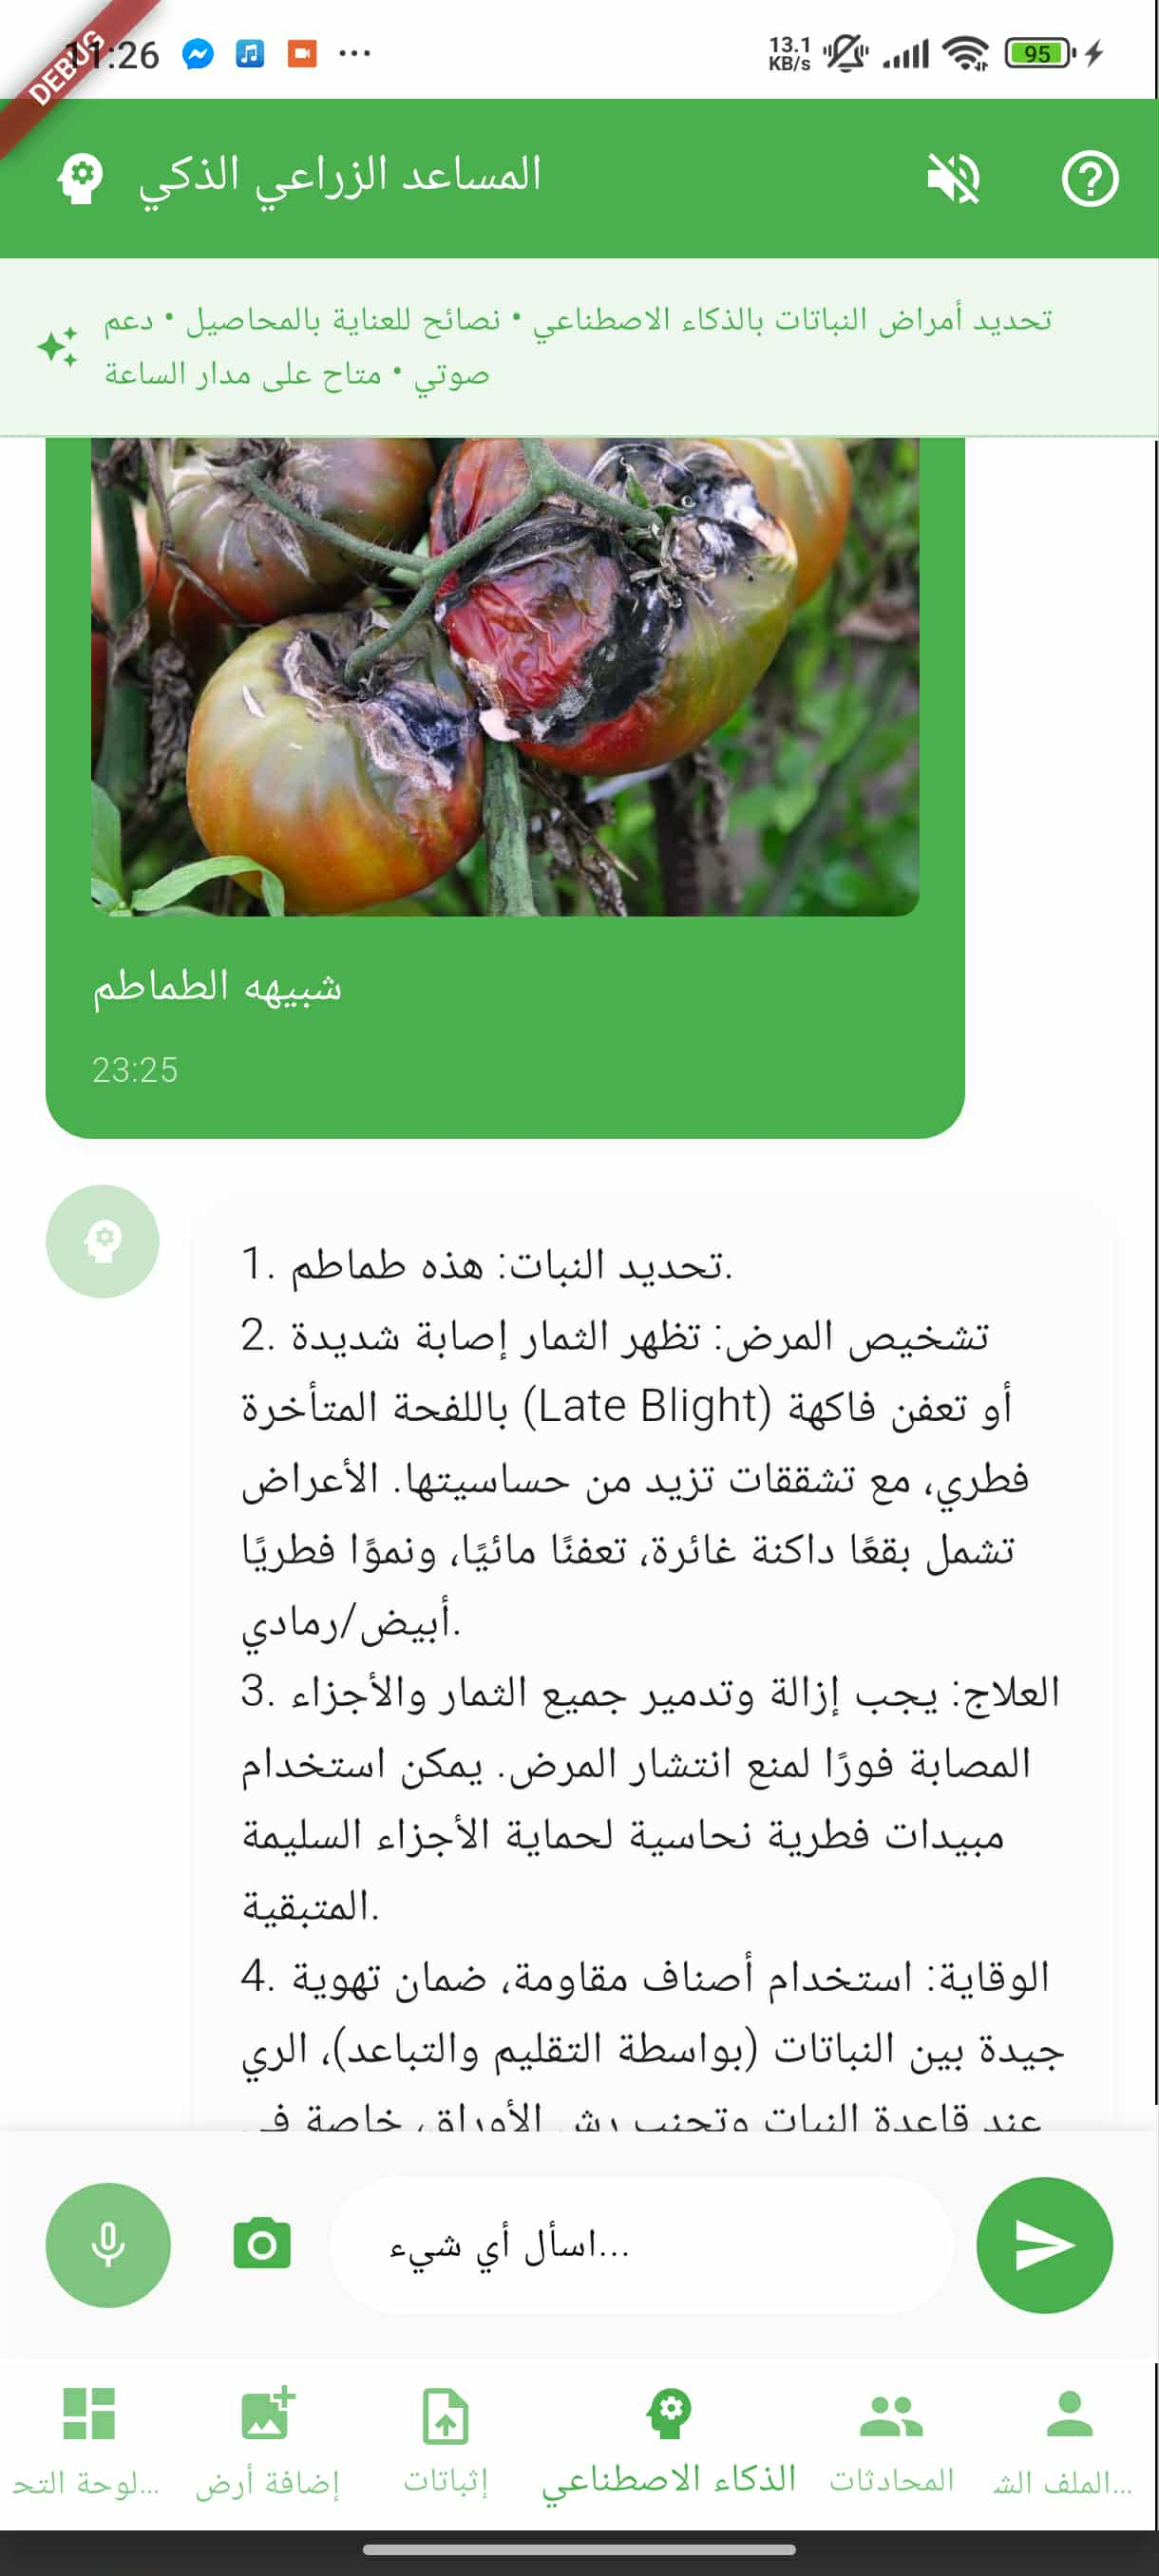
\includegraphics[width=0.9\columnwidth]{images/chatbot.jpg}
\caption{Chatbot Conversation}
\label{fig:architecture}
\end{figure}

This voice-first, multimodal design dramatically reduces barriers to technology adoption, particularly for older women farmers or those with limited digital literacy. The chatbot essentially provides each woman farmer with a personal agricultural extension officer available 24/7—overcoming the historical exclusion of women from male-dominated extension services.

\newpage
\subsection{Analysis of Agricultural Technology Platforms}

A brief overview of several platforms and concepts in the agricultural technology sector, followed by a comparative analysis with emphasis on gender inclusion.

\subsection*{Platform Descriptions}
\begin{description}
    \item[\textbf{Smart Farm}] A general concept for modern farming that integrates technologies like IoT, sensors, and data analytics for precision agriculture. Not designed specifically for smallholder or women farmers; assumes access to capital and technical expertise.

    \item[\textbf{iFarming}] A broad term referring to intensive farming methods or integrated farming systems. Represents an agricultural methodology rather than a specific digital service; typically oriented toward commercial operations.

    \item[\textbf{Seabex}] A focused agritech platform providing AI-driven, sensor-free irrigation recommendations using satellite imagery. Excels at crop monitoring but does not address financial inclusion, gender equity, or investor connections.

    \item[\textbf{Farmcrowdy}] A Nigerian platform that connects investors with farmers to fund agricultural cycles. Operates on a profit-sharing model but does not specifically prioritize women farmers or address gender-specific barriers to agricultural success.

    \item[\textbf{Hrayer}] A comprehensive platform designed specifically to empower rural women farmers by integrating financial services (investor matchmaking with gender priority, profit sharing), operational tools (IoT crop tracking), accessibility features (voice-enabled multilingual chatbot), and community building—all designed to address the unique barriers women face in agriculture.
\end{description}

\subsection*{Feature Comparison Table}

\begin{table}[h!]
\centering
\small
\renewcommand{\arraystretch}{1.3}
\begin{tabular}{l >{\centering\arraybackslash}p{0.6cm} >{\centering\arraybackslash}p{0.9cm} >{\centering\arraybackslash}p{1.55cm} >{\centering\arraybackslash}p{1.0cm}}
\toprule
\textbf{Feature} & Smart Farm & iFarming  & Farmcrowdy & \textbf{Hrayer} \\
\midrule
Gender Focus     & $\times$ & $\times$  & $\times$ & $\checkmark$ \\
Investor Matchmaking     & $\times$ & $\times$  & $\checkmark$ & $\checkmark$ \\
Real-Time IoT Tracking & $\checkmark$ & $\checkmark$ & $\times$ & $\checkmark$ \\
Voice-Enabled Chatbot     & $\times$ & $\times$ & $\times$ & $\checkmark$ \\
Multilingual Support     & $\times$ & $\times$ & $\times$ & $\checkmark$ \\
Impact \& Profit Share     & $\times$ & $\times$ & $\checkmark$ & $\checkmark$ \\
Women's Community     & $\times$ & $\times$ & $\times$ & $\checkmark$ \\
\bottomrule
\end{tabular}
\caption{Comparative view showing Hrayer's unique focus on women's empowerment features}
\label{tab:feature_comparison}
\end{table}

\section{Methodology and System Architecture} \label{sec:methodology}
\subsection{Development Methodology}

The Hrayer platform was developed during a 1-week intensive design sprint with continuous feedback from rural women farmers. Given the compressed timeline and the critical importance of user-centered design for the target population, we employed rapid prototyping methodology focused on delivering a functional minimum viable product (MVP) with core features validated through quick iteration cycles with women farmer representatives.

\subsubsection{Gender-Inclusive Design Principles}

Throughout development, we applied the following principles:
\begin{itemize}
\item \textbf{Simplicity First}: Minimize steps and technical jargon; use visual cues over text
\item \textbf{Voice-First Interaction}: Prioritize audio input/output to overcome literacy barriers
\item \textbf{Cultural Sensitivity}: Design interfaces and language that respect local norms and women's roles
\item \textbf{Offline Capability}: Cache critical information for areas with intermittent connectivity
\item \textbf{Privacy \& Safety}: Implement robust privacy controls recognizing women's unique safety concerns
\item \textbf{Community Features}: Build peer support networks to overcome isolation
\end{itemize}

\subsubsection{Technology Stack}
The platform employs the following technologies:
\begin{itemize}
\item \textbf{Frontend}: Flutter, cross-platform mobile framework enabling simultaneous iOS and Android development with focus on accessibility features
\item \textbf{Backend}: Firebase suite including:
\begin{itemize}
\item Firestore - NoSQL cloud database for user profiles and project data
\item Firebase Authentication - secure user management with phone-number authentication (no email required)
\item Firebase Cloud Messaging - real-time notifications in local languages
\item Imgur - image storage for crop photos and documentation
\end{itemize}
\item \textbf{AI Service}: Google Gemini-2.5-Flash API for multilingual chatbot and image analysis
\item \textbf{IoT Platform}: ESP8266 WiFi-enabled microcontroller modules (pre-configured for easy deployment)
\item \textbf{Communication}: SIM800L GSM module for cellular data transmission from remote farm locations
\end{itemize}

\subsubsection{Development Tools}
\begin{itemize}
\item \textbf{IDEs}: Android Studio and Visual Studio Code
\item \textbf{Design}: Figma for UI/UX mockups with accessibility testing
\item \textbf{Version Control}: Git/GitHub, GitLab for collaborative development
\end{itemize}

\subsubsection{IoT Sensors Designed for Women Farmers}

In the Hrayer ecosystem, ESP8266-based IoT sensor modules are deployed across farmlands to provide real-time environmental monitoring through a mobile-friendly dashboard. Each module integrates multiple sensor types:
\begin{itemize}
\item \textbf{Soil Moisture}: Capacitive soil moisture probes (corrosion-resistant, more durable than resistive sensors)
\item \textbf{Temperature and Humidity}: DHT22 sensors (operating range: -40 to 80°C, ±0.5°C accuracy)
\item \textbf{Light Intensity}: LDR (Light Dependent Resistor) photoresistors for measuring ambient light levels
\item \textbf{Nutrient Analysis}: Nitrate sensors for nitrogen content monitoring (critical for fertilization decisions)
\end{itemize}

Communication Architecture:
Data is transmitted wirelessly via the \textbf{SIM800L GSM module}, which connects directly to cellular networks (2G/GPRS), eliminating dependency on WiFi infrastructure in remote agricultural areas. This design choice ensures:
\begin{itemize}
\item Wide coverage in rural locations without broadband access
\item Independent operation without requiring women farmers to manage internet connectivity
\item Minimal power consumption through periodic data transmission
\item Professional data presentation that builds investor confidence in women-led projects
\end{itemize}

Sensor readings are collected at 30-minute intervals, packaged into JSON payloads, and transmitted to Firebase Realtime Database via HTTP requests. Women farmers receive simple notifications ("Your soil is dry - time to water") rather than raw technical data, while investors can access detailed analytics that demonstrate professional farm management.

\subsection{System Architecture}

The Hrayer platform consists of four primary modules:

\begin{figure}[H]
\centering
% TODO: Create and insert system architecture diagram
\includegraphics[width=0.9\columnwidth]{images/image.png}
\caption{Hrayer platform system architecture showing interaction between farmers, investors, IoT sensors, and backend services.}
\label{fig:architecture}
\end{figure}

\subsubsection{Farmer-Investor Matchmaking Module}

This module implements an intelligent matching algorithm that considers:

\begin{equation}
    \text{Match Score} = w_1 R  + w_2 C + w_3 G
    \label{eq:matching}
\end{equation}

where:
\begin{itemize}
  \item $R$ = Risk profile compatibility
  \item $C$ = Crop type interest
  \item $G$ = Geographic preference
  \item $w_i$ = Weighting factors
\end{itemize}

% TODO: Provide details on matching algorithm implementation
% TODO: Include database schema for user profiles
% TODO: Add verification process for farmers and investors
\subsubsection{Real-Time Crop Monitoring Module}

The Real-Time Crop Monitoring Module leverages IoT sensor networks to provide continuous oversight of crop health. Sensor data is transmitted to a centralized server over HTTP, where algorithms evaluate plant conditions. This system enables instant detection of environmental anomalies and triggers alerts for farmers and agronomists.

Alerts are generated according to predefined thresholds, as described by Equation~\ref{eq:alert}:

\begin{equation}
    \text{Alert} =
    \begin{cases}
    1, & \text{if } \theta < \theta_{\min} \text{ or } \theta > \theta_{\max} \\
    0, & \text{otherwise}
    \end{cases}
    \label{eq:alert}
\end{equation}

where $\theta$ represents the measured soil moisture level, and $\theta_{\min}$ and $\theta_{\max}$ are thresholds determined from historical crop data and agronomic studies. Similar thresholding is applied to other parameters such as temperature, humidity, and nutrient concentration to ensure comprehensive crop health evaluation.

\subsubsection{AI Chatbot Module}

The chatbot employs NLP to understand farmer queries in natural language and provide contextual responses.

% TODO: Specify chatbot architecture (rule-based, retrieval-based, generative)
% TODO: Include sample conversations
% TODO: Add training dataset size and sources
% TODO: Specify supported languages

\subsubsection{Impact \& Profit Sharing Module}

The platform implements a transparent profit distribution mechanism. The total revenue $R$ is first subject to a platform commission $c = 0.05$ (5\%), after which profits are allocated between farmers and investors. Farmer profit depends not only on a base share but also on their contribution in terms of land, materials, water, or tools.

\begin{equation}
    \text{Profit}_{\text{farmer}} = (1 - c) \cdot R \cdot (\alpha + \beta)
    \label{eq:farmer_profit}
\end{equation}

\begin{equation}
    \text{Profit}_{\text{investor}} = (1 - c) \cdot R \cdot (1 - \alpha - \beta)
    \label{eq:investor_profit}
\end{equation}

where:
\begin{itemize}
    \item $c = 0.05$ is the platform commission (5\% of total revenue),
    \item $\alpha = 0.20$ is the base farmer share (20\% of post-commission revenue),
    \item $\beta$ is an additional share awarded to the farmer based on their contribution of land, materials, water, and tools,
    \item $\text{Profit}_{\text{investor}}$ is distributed among investors proportionally to their investment amounts.
\end{itemize}

This dynamic allocation ensures fairness: farmers who provide more resources receive a higher profit share, while investors are rewarded proportionally to their financial contributions. The system can be configured through automated dashboards to reflect contribution weights, ensuring transparency and trust among all stakeholders.

% TODO: Include profit-sharing agreement template
% TODO: Add legal/regulatory compliance details


\section{Implementation and Key Features} \label{sec:implementation}

\subsection{User Interface Design}

The platform features separate interfaces optimized for farmers and investors:

% TODO: Insert screenshots of farmer mobile app
% TODO: Insert screenshots of investor dashboard
% TODO: Include UX research findings if available

\begin{figure}[H]
\centering
% TODO: Insert farmer app screenshot
\includegraphics[width=0.4\columnwidth]{images/farmer_dash.jpg}
\caption{Farmer mobile application interface.}
\label{fig:farmer_ui}
\end{figure}

\begin{figure}[H]
\centering
% TODO: Insert investor dashboard screenshot
\includegraphics[width=0.4\columnwidth]{images/sponso.jpg}
\caption{Investor dashboard showing portfolio and crop monitoring.}
\label{fig:investor_ui}
\end{figure}

\subsection{Core Features Implementation}

\subsubsection{Smart Funding Platform}

Farmers create detailed project proposals including:
\begin{itemize}
  \item Crop type and planting plan
  \item Required funding amount
  \item Expected timeline and yield
  \item Farmer credentials and land documentation
  \item Historical performance (if available)
\end{itemize}

\subsubsection{Real-Time Progress Tracking}

Investors receive automated updates on:
\begin{itemize}
  \item Crop growth stages with images
  \item Environmental conditions
  \item Potential risks or interventions needed
  \item Expected harvest timeline
\end{itemize}

\subsubsection{Instant Agricultural Assistance}

The chatbot provides guidance on:
\begin{itemize}
  \item Pest and disease identification
  \item Weather-appropriate farming practices
  \item Fertilizer and irrigation recommendations
  \item Market price information
  \item Best practices for crop-specific challenges
\end{itemize}

\section{Target Market and Competitive Analysis} \label{sec:market}

\subsection{Target Market Segmentation}

\subsubsection{Primary Users: Farmers}

\begin{itemize}
  \item \textbf{Demographics}: All farmers who lack financial support to use their land.
  \item \textbf{Geographic Focus}: Farmers who are in tunisia's rural areas.
  \item \textbf{Crop Types}: Seasonal crops (2-6 months long investment).
  \item \textbf{Technology Access}: Smartphone
\end{itemize}

\subsubsection{Secondary Users: Investors}

\begin{itemize}
  \item Individual impact investors
  \item Agricultural cooperatives
  \item Microfinance institutions
  \item Corporate social responsibility programs
  \item Development agencies
\end{itemize}

\subsection{Market Opportunity}

\section{Business Model and Revenue Strategy} \label{sec:business}

\subsection{Revenue Model}

Hrayer generates revenue through multiple streams:

\begin{enumerate}
  \item \textbf{Transaction Commission}: 5\% commission on all successful investments and profit distributions.
  \item \textbf{Farmer-Investor Profit Sharing}:
    \begin{itemize}
        \item $c = 0.05$ is the platform commission (5\% of total revenue),
        \item $\alpha = 0.20$ is the base farmer share (20\% of post-commission revenue),
        \item $\beta$ is an additional share awarded to the farmer based on their contribution of land, materials, water, and tools,
        \item $\text{Profit}_{\text{investor}}$ is distributed among investors proportionally to their investment amounts.
    \end{itemize}
  \item \textbf{IoT Hardware Sales/Leasing}:
    \begin{itemize}
      \item Farmers can buy or lease IoT sensor kits (soil moisture, temperature, humidity, nutrient sensors, GSM module)
      \item Leasing model: \$5–\$10/month per plot depending on sensor package
    \end{itemize}
  \item \textbf{Data Analytics Services}:
    \begin{itemize}
      \item B2B offering to agribusinesses, cooperatives, and government agencies
      \item Includes predictive yield reports, market demand forecasts, and soil health trends
    \end{itemize}
  \item \textbf{Partnership Commissions}:
    \begin{itemize}
      \item Commissions from agricultural input suppliers (seeds, fertilizers, equipment)
      \item Insurance providers for crop coverage
    \end{itemize}
\end{enumerate}

\subsection{Marketing and Sales Strategy}

\subsubsection{Sales Strategy}

\begin{itemize}
  \item \textbf{Direct Sales}: Field agents visit agricultural regions to onboard farmers and explain profit-sharing and IoT monitoring benefits.
  \item \textbf{Partnership Channel}: Collaborate with agricultural cooperatives, NGOs, and farmer associations.
  \item \textbf{Digital Marketing}: Social media campaigns (Facebook, Instagram, LinkedIn) and online ads targeting farmers and investors.
  \item \textbf{Farmer-Investor Engagement}: Emphasize transparent profit-sharing (20\% base + contribution-based extra for farmers; proportional distribution for investors) to build trust and adoption.
\end{itemize}

\subsubsection{Communication Strategy}

\begin{itemize}
  \item \textbf{Social Media Campaigns}: Facebook, Instagram, LinkedIn, and YouTube to reach both rural farmers and urban investors.
  \item \textbf{Influencer Marketing}: Agricultural experts, local agronomists, and rural community leaders to promote platform adoption.
  \item \textbf{Traditional Media}: Local radio, newspapers, and TV advertising in farming regions to increase trust and visibility.
  \item \textbf{Direct Engagement}: On-site workshops, product demonstrations, and training sessions for farmers and investors.
  \item \textbf{Strategic Partnerships}: Collaborations with cooperatives, NGOs, and government agricultural programs to accelerate adoption.
\end{itemize}

\section{Results and Validation} \label{sec:results}

\subsection{Current Accomplishments}

\subsubsection{Technical Milestones}

\begin{itemize}
  \item Platform architecture implemented
  \item IoT sensor network deployed MVP (Temperature, Humidity and server updates)
  \item Chatbot (using gemini for now)
  \item Mobile applications developed
\end{itemize}

\subsection{Contribution to Sustainable Development Goals}

Hrayer contributes to multiple UN SDGs:

\begin{itemize}
  \item \textbf{SDG 1 (No Poverty)}: Increases farmer income through better access to capital
  \item \textbf{SDG 2 (Zero Hunger)}: Improves food security through optimized agriculture
  \item \textbf{SDG 8 (Decent Work)}: Creates economic opportunities in rural areas
  \item \textbf{SDG 9 (Innovation)}: Promotes agricultural innovation and infrastructure
\end{itemize}

\section{Roadmap and Future Work} \label{sec:conclusion}

\subsection{Development Roadmap}

The Hrayer platform will evolve through four strategic phases:

\subsubsection{Phase 1: 2025 - Initial Deployment}

\begin{itemize}
  \item Launch platform in pilot region (Kasserine, Kef and Gafsa)
  \item Deploy IoT sensors in 20-30 farms
  \item Onboard 10 farmers and investors
  \item Validate core features and gather feedback
  \item Achieve profitability in pilot market
\end{itemize}

\subsubsection{Phase 2: 2025-2026 - Feature Enhancement}

\begin{itemize}
  \item Improve AI chatbot with expanded knowledge base
  \item Add weather prediction integration
  \item Implement insurance product offerings
  \item Develop agricultural input marketplace
  \item Expand sensor network capabilities
  \item Introduce advanced analytics dashboard
\end{itemize}

\subsubsection{Phase 3: 2026-2028 - Regional Expansion}

\begin{itemize}
  \item Scale to other tunisian regions
  \item Partner with regional agricultural organizations
  \item Expand IoT infrastructure
  \item Reach 500 total farmers
\end{itemize}

\subsubsection{Phase 4: 2028-2029 - International Growth}

\begin{itemize}
  \item Expand to international markets
  \item Establish partnerships with global agricultural development organizations
  \item Implement continuous innovation approach
  \item Develop API for third-party integrations
  \item Launch B2B agricultural data services
\end{itemize}

\subsection{Technical Enhancements}

Future technical developments include:

\begin{itemize}
  \item Satellite imagery integration for large-scale monitoring
  \item Machine learning models for yield prediction
  \item Automated irrigation control systems
  \item Drone integration for crop surveillance
\end{itemize}
\subsection{Research and Innovation}

Ongoing research areas:

\begin{itemize}
  \item Optimal sensor placement algorithms
  \item Crop disease prediction models
  \item Dynamic profit-sharing optimization
  \item Agricultural supply chain integration
  \item Climate resilience strategies
\end{itemize}

\subsection{Summary of Contributions}

Hrayer represents a comprehensive solution to agricultural financing and knowledge gaps by:

\begin{itemize}
  \item Creating transparent farmer-investor relationships
  \item Providing real-time crop monitoring through IoT
  \item Delivering instant expert guidance via AI
  \item Implementing fair profit-sharing mechanisms
  \item Contributing to sustainable development goals
\end{itemize}

\subsection{Expected Impact}

Successful deployment of Hrayer is expected to:

\begin{itemize}
  \item Increase farmer income
  \item Improve crop yields by 100\% through optimized farming
  \item Reduce agricultural risks through early warning systems
  \item Create direct and indirect jobs for women and farmers
  \item Facilitate in agricultural investments annually
\end{itemize}
\end{document}